\documentclass{article}

% if you need to pass options to natbib, use, e.g.:
%     \PassOptionsToPackage{numbers, compress}{natbib}
% before loading neurips_2019

% ready for submission
% \usepackage{neurips_2019}

% to compile a preprint version, e.g., for submission to arXiv, add add the
% [preprint] option:
\usepackage[preprint]{neurips_2019}

% to compile a camera-ready version, add the [final] option, e.g.:
%  \usepackage[final]{neurips_2019}

% to avoid loading the natbib package, add option nonatbib:
%     \usepackage[nonatbib]{neurips_2019}

\usepackage[utf8]{inputenc} % allow utf-8 input
\usepackage[T1]{fontenc}    % use 8-bit T1 fonts
\usepackage{hyperref}       % hyperlinks
\usepackage{url}            % simple URL typesetting
\usepackage{booktabs}       % professional-quality tables
\usepackage{amsfonts}       % blackboard math symbols
\usepackage{nicefrac}       % compact symbols for 1/2, etc.
\usepackage{microtype}      % microtypography

% SHi-ON packages
% argmin argmax begin
\usepackage{amsmath}
\DeclareMathOperator*{\argmax}{arg\,max}
\DeclareMathOperator*{\argmin}{arg\,min}
% argmin argmax end
\newcommand{\norm}[1]{\left\lVert#1\right\rVert}        % norm using amsmath


\title{Adversarial State Aggregation}

% The \author macro works with any number of authors. There are two commands
% used to separate the names and addresses of multiple authors: \And and \AND.
%
% Using \And between authors leaves it to LaTeX to determine where to break the
% lines. Using \AND forces a line break at that point. So, if LaTeX puts 3 of 4
% authors names on the first line, and the last on the second line, try using
% \AND instead of \And before the third author name.

\author{%
Authors \\ %\thanks{Use footnote for providing further information
%    about author (webpage, alternative address)---\emph{not} for acknowledging
%    funding agencies.}%
Department of Computer Science\\
University of New Hampshire \\
\texttt{\{authors\}@cs.unh.edu} \\
% examples of more authors
% \And
% Coauthor \\
% Affiliation \\
% Address \\
% \texttt{email} \\
% \AND
% Coauthor \\
% Affiliation \\
% Address \\
% \texttt{email} \\
% \And
% Coauthor \\
% Affiliation \\
% Address \\
% \texttt{email} \\
% \And
% Coauthor \\
% Affiliation \\
% Address \\
% \texttt{email} \\
}

\begin{document}

    \maketitle

    \begin{abstract}
        Promising advances in deep reinforcement learning suggests several application to the algorithms. However
        robustness of these algorithms remains doubts to trust these algorithms in practice. In this paper we study
        resistance of the state-of-the-art algorithms to environment dynamics. We then show the amount of robustness
        we can achieve as a guarantee of performance in presence of those changes.
    \end{abstract}


    \section{Introduction}
    Real-world problems embody high-dimensional state spaces where in computational issues
    arise.
    Various approximation methods are proposed in the literature to reduce the resulted value function
    dimensionality \cite{Sutton1998, Francois-Lavet2018}.
    State aggregation is one of the simplest and most analytically transparent state representation approximation.

    Although state aggregation may not generalize as well as neural network-based methods, the techniques has both
    analytical and practical advantages \cite{Lagoudakis2003}.
    In comparison, state aggregation takes less computation power to calculate representative features.
    Moreover, analysis and troubleshooting in a state aggregation process is more obvious than a black-box neural
    network.
    Approximation is a corner stone in all successful RL methods to hold a "good" mapping between a large state
    space to a much smaller one where in value function is computable or at least feasible.
    These "good" approximators can end up with "good" features to represent the projected state space.

    The cross-fertilization in using state aggregation and deep neural networks in solving immense state
    space problems in RL is also profound.
    While the newly emerged methods are growing at a staggering pace, a parallel area of research has been formed
    wherein a variety of techniques have been utilized to make these methods contravene their promised functionality.
    These efforts would be served to develop robustness in those spectacular models and reduce their
    susceptibility to data tampering or dynamics of the environment.

    In this work, we scrutinize state-of-the-art deep RL algorithms resiliency to environment parameters alterations
    and then introduced our approach to overcome those. Then a guarantee of performance to these attacks is introduced.


    \section{Method}
    For the sake of clarity, we elaborate on some preliminary definitions here to have a consistent set of notations
    to the end of this paper. We use model-free LSPI and LSTDQ \citep{Lagoudakis2003} to update and
    evaluate the policy of actions, respectively. CRAAM, on the other hand, as a exact method tries to approximate
    the value function by dynamic programming optimization.

    We developed an aggregation scheme to lower the state space dimensionality by assigning same action to the state
    in a neighbourhood, so called nearest neighbour/ piecewise linear aggregation.


    \subsection{Adversarial attacks}
    The designed attack may have different levels of access to the underlying training policy which have motivated
    the community to classify adversarial attacks into two distinct categories, namely \textit{white-box} or
    \textit{black-box} attacks. White-box attacks illustrating the scenario in which the... Adversarial attacks fall
    in either one of the following categories based upon the stage, which in the adversary perturbs the model:
    \begin{itemize}
        \item Train time: Data poisoning.
        \item Evaluation time: Adversarial examples.
        \item Deploy time: Black-box attacks.
    \end{itemize}


    \subsection{Objective}
    The aggregate problem is stochastic even if the original problem is deterministic. Once we lay out the aggregate
    problem framework we can solve the problem by any exact methods either value- or policy-space solutions.


    The ultimate goal is deceiving the model either in choosing the worst possible action in an RL task or misclassifying an input in a classification task in a way which is not perceptible for unaided eye. In terms of a Markovian RL task we show how minimum set of worst-case actions are needed to result in the minimum final reward. We try to show that the model is not robust to other configuration of each benchmarks with different dynamics.

    The main goal of adversarial training and examples can be expressed briefly in form of the following equation:
    %    \begin{equation}
    %        \begin{aligned}
    %            & \underset{\theta}{\min}
    %            & & \sum_{x,y \in S} \underset{\delta \in \Delta}{\max}
    %            & & & \textbb{Loss}(x + \delta, y; \theta)
    %        \end{aligned}
    %    \end{equation}

    \section{Devising Adversarial Attacks}
    Neural networks are vulnerable to adversarial attacks either in supervised learning or reinforcement learning settings \cite{Huang2017}. Such weakness could possibly result in unrecognizable differences for the unaided eye in the presence of perturbation which leads to misclassification for neural network based model \cite{Szegedy2014, Goodfellow2014}.


    \subsection{Observation-perturbed attacks}


    where in we trying to find an adversarial example (inner maximization) in order to adversarially train a robust model (outer minimization).

    We define $s_\eta$ as the perturbed observation:
    \begin{equation}
        s_\eta = s . (1 + \epsilon)
    \end{equation}


    Let $s_\eta$ be the perturbed observation and $s_c$ scaled observation, so we are trying to find the following:
    \begin{equation}
        \begin{aligned}
            & \underset{s}{\argmin}
            & & {\norm{s_\eta - s_c}} = \norm{s . (1 + \epsilon) - s_c}
        \end{aligned}
    \end{equation}
    which is the state observation that have the minimum distance between real-world [scaled] observation and the perturbed one.

    In order to expand the applicability of designed adversarial attacks to an assortment of algorithms [models], we rely on \textit{transferability property} of RL-specific adversarial attacks \cite{Szegedy2014, Papernot2016, Goodfellow2014a}. \cite{Huang2017} clearly assert [or asserts?!] attacks are deployable to a group of trained RL models aimed at the same task.

    \subsection{Reward-Perturbed attacks}
    In an adversarial environment we try to perturb reward to interfere in learning process of the RL agent. We considered this attack also in scenarios with a single reward which we will show the process later.

    \section{Experiment}
    We apply the approach to two MDPs proposed by\cite{Strehl2004}. \textit{RiverSwim} an MDP consists of six states and \textit{SixArms} one with seven states. In \textit{RiverSwim} flow of the river is to left and the swimmer picks probabilistically equal either state 1 or 2 as the start point. All states but two terminal states have zero reward to land at while the right most one rewards substantially higher than the other one. The agent in SixArms selects between six distinct actions which pulls different arms of a multi-armed bandit. By pulling an arm the agent traverses to a new state. Although the agent does not obtain reward by pulling the arms but going to the connected state to that arm is highly rewarding in which the transition probability is in inverse relationship with the reward value.

    As both problems favor keeping the agent in states with lower reward, exploration is paramount to maximize the accumulated reward. This is also confirmed by the authors in \cite{Strehl2004} that the agent will fail to learn when a rudimentary $\epsilon$-greedy algorithm.

    Our implementation uses Deep Q-Network (DQN)\cite{Mnih2015} as the policy optimizer. OpenAI Gym \cite{Brockman2016} is the testbed in the benchmarks in this paper. In training phase, models are trained in the environment. Online methods such as DQN learn by interacting directly in the environment, however, CRAAM

    % \begin{figure}
    %     \centering
    %     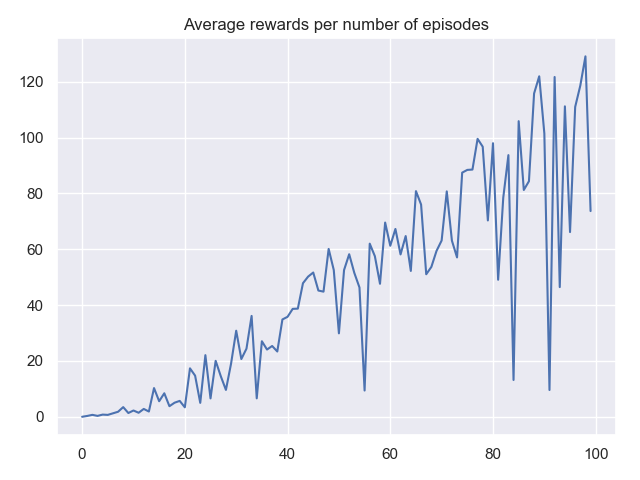
\includegraphics[width=1\columnwidth]{minutia/cartpole-v1_batchsize-32_episodes-100_full-step.png}
    %     \caption{Average reward of DQN training to 100 episodes in cartpole.}
    %     \label{fig:my_label}
    % \end{figure}



    \section{Future Works}
    We developed the presented approach with having reproducibility in mind. It could be served as a launching pad for the future contributors who want to surf this newly emerged field deeper. Future ideas to pursue is a generative model to be able to generate adversaries from a network.

    \section*{Appendix}

    \subsection{Implementation note}
    * Reshape is needed after getting each state from Gym models.




    \bibliographystyle{plain}
    \bibliography{library}
    % \section*{References}



    % [1] Alexander, J.A.\ \& Mozer, M.C.\ (1995) Template-based algorithms for
    % connectionist rule extraction. In G.\ Tesauro, D.S.\ Touretzky and T.K.\ Leen
    % (eds.), {\it Advances in Neural Information Processing Systems 7},
    % pp.\ 609--616. Cambridge, MA: MIT Press.

    % [2] Bower, J.M.\ \& Beeman, D.\ (1995) {\it The Book of GENESIS: Exploring
    %   Realistic Neural Models with the GEneral NEural SImulation System.}  New York:
    % TELOS/Springer--Verlag.

    % [3] Hasselmo, M.E., Schnell, E.\ \& Barkai, E.\ (1995) Dynamics of learning and
    % recall at excitatory recurrent synapses and cholinergic modulation in rat
    % hippocampal region CA3. {\it Journal of Neuroscience} {\bf 15}(7):5249-5262.

\end{document}
